\chapter{A view of the EoR window from the HERA-19 commissioning array}
\label{chapter:eor_window_HERA}

As emphasized in Chapter~\ref{chapter:eor_window_paper32img}, it is important to constrain intrinsic and leaked polarized signal for any EoR experiment. The objective of this Chapter was an exploration of eight nights of data from the Hydrogen Epoch of Reionization Array (HERA) 19-element commissioning array, coupled with simulations of the instrument, in order to forecast how much of a problem polarization would pose for this interferometer. 
This work also represents the first power spectral analysis from HERA. While not in the realm of an EoR-level integration, we were able to offer some initial expectations for this new instrument's performance in the Fourier domain.

This work is organized as follows: in Section~\ref{sec:hera19_leak} we review the theory behind polarization leakage into unpolarized signal and simulate the effect for a model of HERA. In Section~\ref{sec:hera19_obs} we describe the HERA data that we used, its calibration and reduction to power spectra. We present our results, and discuss the implications for HERA's EoR measurements, in Section~\ref{sec:hera19_results}, and conclude in Section~\ref{sec:hera19_conc}. We assume the cosmological parameters reported by \cite{Planck.16} throughout.

\section{Polarization Leakage Simulations}
\label{sec:hera19_leak}


\section{Observations \& Reduction}
\label{sec:hera19_obs}

In this work we used eight nights of observations from the HERA-19 commissioning array. HERA is a low-frequency interferometer composed of 14\,m-diameter dishes arranged in a close-packed hexagonal array of 14.7\,m spacing. The commissioning array consists of nineteen dishes (see Figure~\ref{fig:hera19_antpos}); HERA is being constructed in staged build-outs, and upon completion will consist of 350 dishes in a fractured hexagon configuration \citep[see][]{Dillon.16, deBoer.17}. A feed cage containing two dipole feeds (recycled from the PAPER array, see \citealt{Parsons.10}), oriented in North-South and East-West directions, is suspended above each dish \citep{Neben.16}.

HERA only observes in drift-scan mode. The observations we used were eight nights, from Julian Date (JD) 2457548 to 2457555; LSTs 10.5 -- 23 hr. Drift-scan visibilities were recorded every 10.7 seconds for 1024 evenly-spaced channels across the 100-200\,MHz bandwidth. These data were divided into {\sc miriad} data sets roughly 10 minutes long. A night's observation lasted 12 hours in total (6pm to 6am South African Standard Time; SAST); of these we used the central 10 hours, to avoid thermal effects of the Sun.

\begin{figure}
\centering
\hspace{-0.5cm}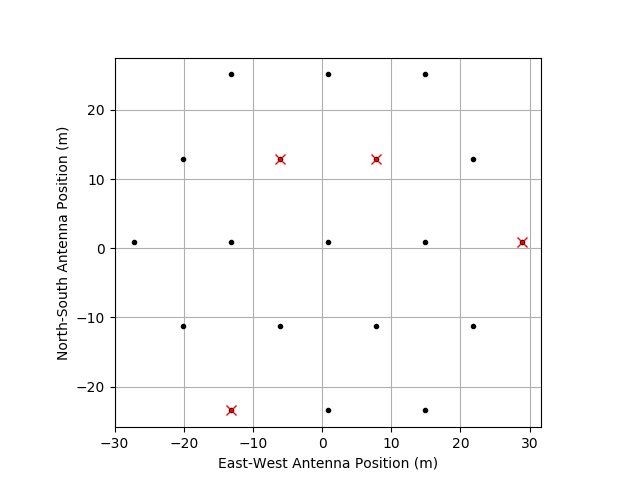
\includegraphics[scale=0.6]{chapters/eor_window_HERA/figures/antpos_hera19.png}
\caption[The centroid position of each dish in the HERA-19 array.]{The centroid position of each dish in the HERA-19 array.  A red "X" marks antennae that were malfunctioning during preprocessing and calibration, and were excluded from further analysis.}
\label{fig:hera19_antpos}
\end{figure}

To identify samples contaminated by radio frequency interference (RFI), a two-dimensional median filter in time and frequency was applied to the visibility data to smooth out high pixel-to-pixel variations, and remove significant outliers that were likely unphysical. The variance of the resulting data was computed, and points with a $z$-score greater than 6 (i.e., points where the value is more than 6$\sigma$ away from the mean) were flagged as initial seeds for RFI extraction. A two-dimensional watershed algorithm was applied using these seeds as starting points, enlarging the regions of RFI-contamination to neighboring pixels with z-scores greater than 2, until all such pixels were flagged. Figure~\ref{fig:hera19_rfi} shows the fractional RFI flag occupancy per time (displayed in LST) and frequency across the 8 days of observations. The majority of the band is relatively clear of RFI. Some clear features are: the FM radio band (below 120 MHz), ORBCOMM satellite communications (137 MHz), an ISS downlink (150 MHz) and VHF TV channels (above 170 MHz)
\footnote{For an extended discussion of RFI as seen by HERA, see Chapter~\ref{chapter:data_prep_and_proc}.}. 
The Galaxy, when transiting zenith at LST$\approx$17.75, is so bright that it appears to degrade our ability to flag RFI.

\begin{figure}
\centering
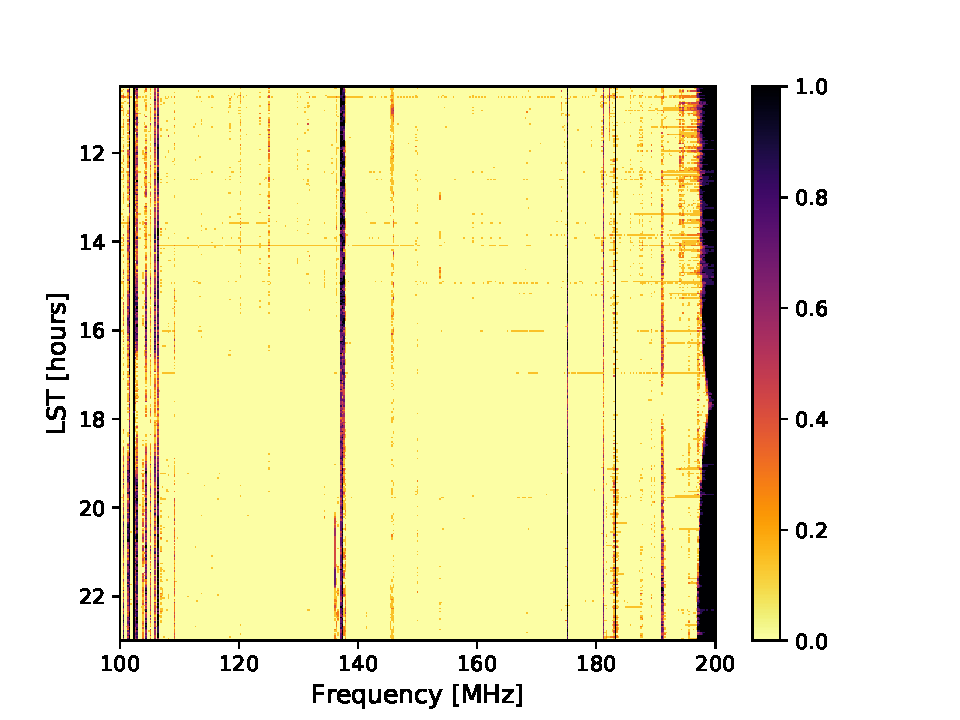
\includegraphics[scale=0.6]{chapters/eor_window_HERA/figures/frac_occ.pdf}
\caption{Fractional RFI flag occupancy per time and frequency over the eight days of observations.}
\label{fig:hera19_rfi}
\end{figure}

\subsection{Calibration}
\label{subsec:hera19_cal}
To perform calibration in {\tt CASA} \citep{casa}, we converted between {\sc miriad} and {\sc uvfits} file formats using {\sc pyuvdata} \citep{pyuvdata}. {\sc uvfits} files could be ingested by {\sc CASA}.

Using LSTs in which the Galactic center (GC; $\alpha, \delta$ = 17h 45m 40.04s,​ ​-29d 0m 28.12s) was transiting, we built a CLEAN model which modelled the GC as an unpolarized point source of strength 1 Jy and flat spectrum, which could be scaled appropriately later (see Equation~\ref{eq:freq_scale}). Clearly, this was an incomplete calibration model. However, as the objective of this work was to explore the response of the instrument in power spectrum space: that is, not combining baselines of different lengths, most of the purpose of the calibration is correcting an initial large cable delay per antenna. Treating the GC as unpolarized is also adequate for this study. The large optical depth towards the GC \citep{Oppermann.12} results in large amounts depolarization in the plane of the Galaxy \citep{Wolleben.06}. Moreover, we expect non-negligible amounts of beam depolarization from the instrument \citep{Neben.16}.

We used the {\tt CASA} {\tt gaincal} and {\tt bandpass} functions to obtain frequency-dependent phase and amplitude solutions for each antenna and dipole arm. Four antennae had very deviant solutions, and their inclusion resulted in low-quality quality images. These were omitted from further analysis (and are marked with red "X"s in Figure~\ref{fig:hera19_antpos}).  Before calibration, we manually flagged the edges of the band (below 110 MHz and above 190 MHz), where spectral behavior is dominated by the high and low pass filtering in the HERA signal chain \citep{deBoer.17}.

Dirty images after calibration are shown in Figure~\ref{fig:hera19_GCimage}. These are multi-frequency synthesis images, where we used all unflagged frequencies on either side of the band edges; 115 MHz to 188 MHz. As expected for a compact array, the Stokes I images capture only the large-scale structure of the Galactic plane. 

\begin{figure}
\centering
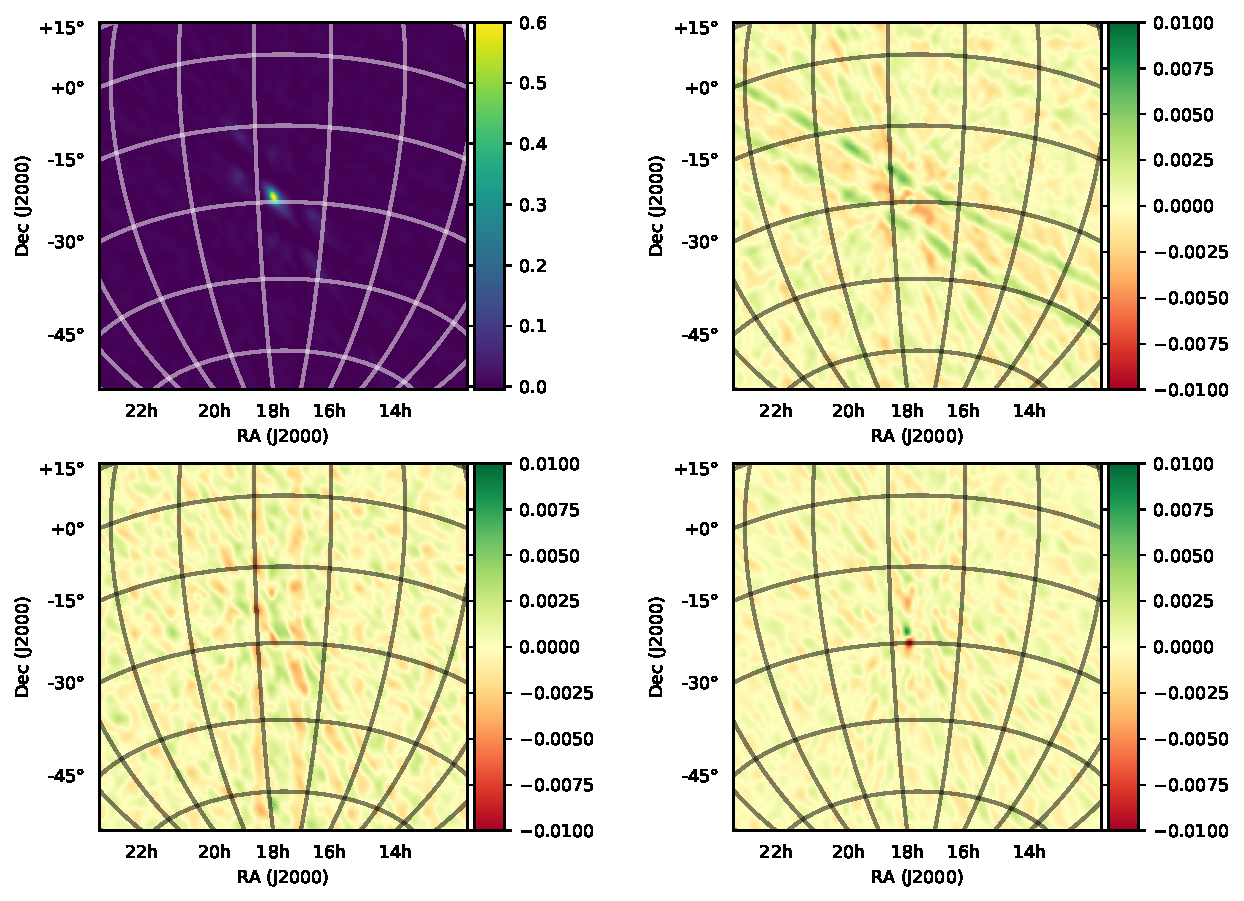
\includegraphics[width=0.9\textwidth]{chapters/eor_window_HERA/figures/galcen.pdf}
\caption[Multi-frequency synthesis images of the Galactic Center (our calibrator source) on JD 2457548 in Stokes I, Q, U and V.]{
Multi-frequency synthesis images of the Galactic Center (our calibrator source) on JD 2457548 in Stokes I, Q, U and V (\textit{top left, top right, lower left, lower right}). 
The colorbar is in units of Jy/Beam (relative to the 1 Jy source model; visibilities were later scaled according to Equation~\ref{eq:freq_scale}).
A separate color scale is used for Stokes I for suitable dynamic range. An R.A., Dec. grid is shown, illustrating the wide-field nature of HERA observations.
}
\label{fig:hera19_GCimage}
\end{figure}

Example bandpass solutions from JD 2457548 are shown in Figure~\ref{fig:hera19_bandpass}. Although some residual RFI remains obvious, the bandpass is smooth and should therefore not couple significant amounts foreground signal into the EoR window.

\begin{figure}
\centering
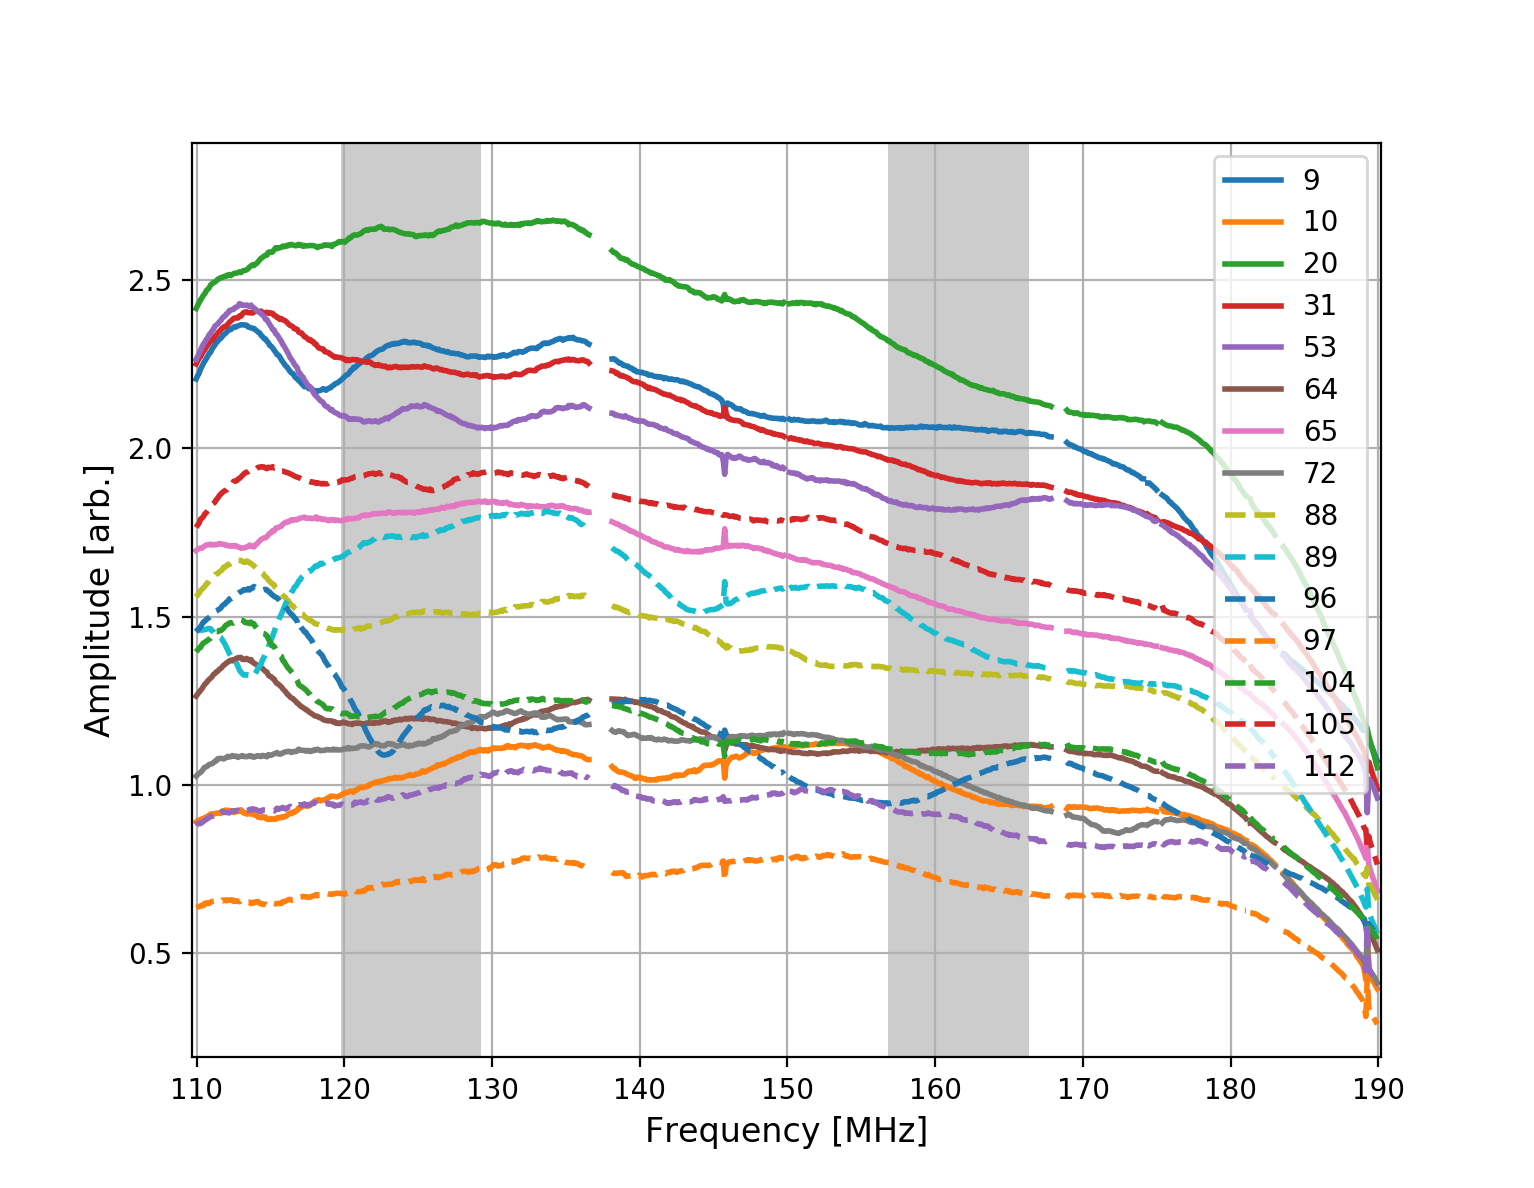
\includegraphics[width=0.9\textwidth]{chapters/eor_window_HERA/figures/h19_2457458_abs_smallzoom.png}
\caption[Bandpass solutions for the North-South dipole orientation obtained for the functioning antennae in the array on JD 2457548.]{Bandpass solutions for the North-South dipole orientation obtained for the functioning antennae in the array on JD 2457548. Antennae are numbered according to their position in the final, 350-element array, leading to apparent out-of-order numbering for the commissioning array. Shaded regions indicate the sub-bands used for power spectrum analysis.}
\label{fig:hera19_bandpass}
\end{figure}

The complex gain solutions were subsequently applied to the {\sc miriad} files. Figure~\ref{fig:hera19_phasecal} shows the effect of calibration on visibilities three nominally redundantly-spaced baselines. Shown in that figure are the phases of three $V_{nn}$ visibilities from 14.7\,m baselines before and after calibration. There were no shared antennae between the visibilities shown. Our calibration was sufficient to enforce redundancy between these nominally-redundant baselines, which granted some verification of our methods.

\begin{figure}
\centering
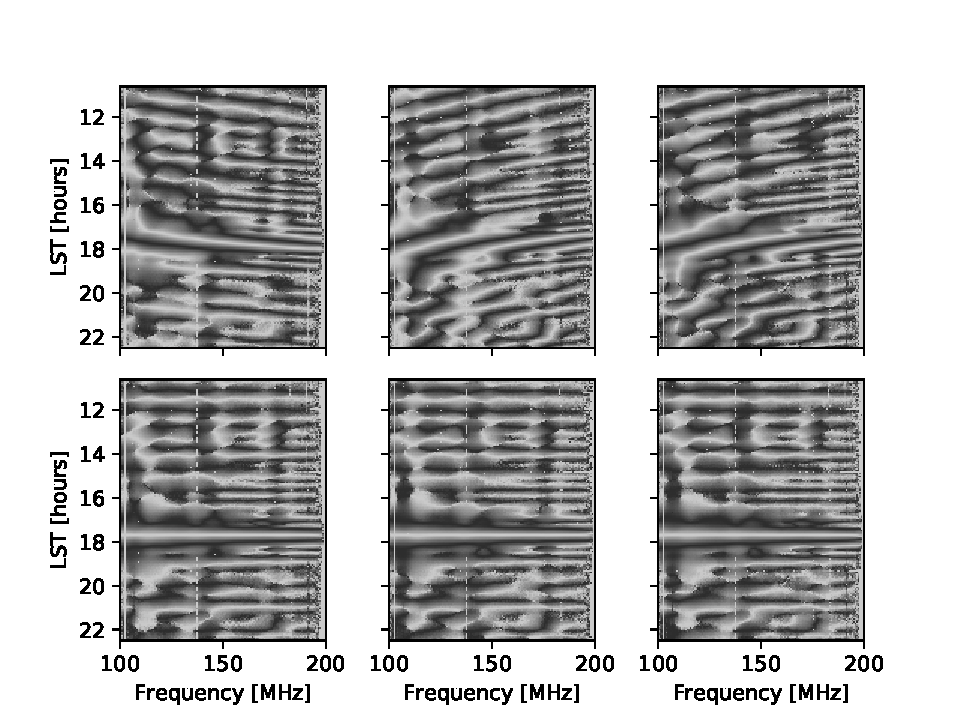
\includegraphics[width=0.9\textwidth]{chapters/eor_window_HERA/figures/phases_pre_post_abscal_h19_cyclic_grey.pdf}
\caption[The effect of calibration on the phases of visibilities from three redundantly-spaced 14.7\,m baselines.]{The effect of calibration on the phases of visibilities from three redundantly-spaced 14.7\,m baselines; \textit{nn} polarization. The color scale is cyclic; black is $\pm\pi/2$ and white is 0 and $\pm\pi$. \textit{Above}: before calibration; \textit{below}: after calibration. A simple sky model was sufficient to enforce redundancy for redundant baselines.}
\label{fig:hera19_phasecal}
\end{figure}

We did not attempt to calibrate \textit{D}-terms in this work as there were no polarized sources identified at low frequencies in the field surveyed, which are required for \textit{D}-term calibration. This limited our interpretive power, which we discuss in Section~\ref{sec:hera19_results}.

We down-selected to two relatively RFI-free 10 MHz sub-bands; 120 to 130 MHz and 157 to 167 MHz, henceforth referred to the ``low band" and the ``high band". These thinner bands are representative of the range of frequencies one could use to claim an EoR detection, since the {\sc hi} signal would be coeval over such a redshift range \citep{Furlanetto.06}. As shown in Figure~\ref{fig:hera19_rfi}, they are both relatively clear of RFI.
The instantaneous \textit{uv}-coverage of the whole band is shown in blue in Figure~\ref{fig:uv-coverage}, with the low and high bands shown in yellow and red, respectively.

\begin{figure}
\centering
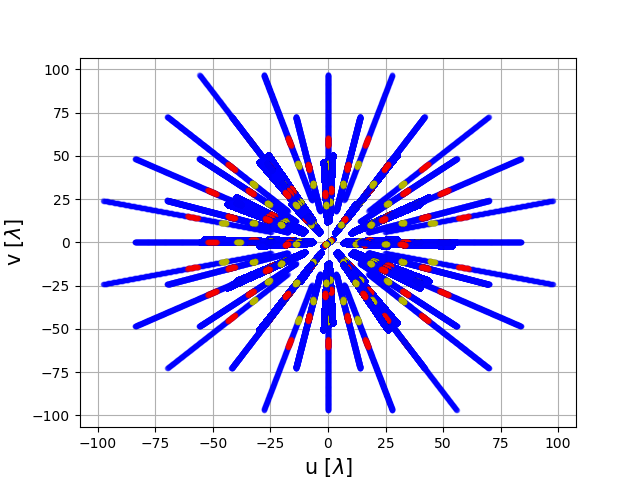
\includegraphics[scale=0.5]{chapters/eor_window_HERA/figures/uvcoverage_hera19-hilo.png}
\caption[The instantaneous \textit{uv}-coverage of the array.]{The instantaneous \textit{uv}-coverage of the array. The \textit{uv}-coverage of the full band, used for calibration and imaging, is shown in blue. The \textit{uv}-coverage high and low bands are shown in red and yellow, respectively.}
\label{fig:uv-coverage}
\end{figure}

Pseudo-Stokes visibilities were formed from the instrumental polarizations. These visibilities were then scaled to the appropriate amplitude using the power law

\begin{equation}
S_{\rm Sgr A^*}(\nu) =  3709 {\rm\, Jy} \times (\nu/408 {\rm \,MHz})^{-2.5}
\label{eq:freq_scale}
\end{equation}

which is drawn from the Haslam map \citep{Haslam.81, Haslam.82, Remazeilles.15}.

\subsection{Forming power spectra}
\label{subsec:pspec}
Power spectra were formed according to the method used in \cite{Pober.13}, \cite{Kohn.16} and Chapter~\ref{chapter:eor_window_paper32img}, which we briefly review here. All Fourier transforms were windowed using a Blackman-Harris window at the center of the sub-band, which minimized sidelobes. \cite{Parsons.12a} define the delay transform as the Fourier transform of a visibility for baseline $ij$ and pseudo-Stokes parameter $P$ along the frequency axis

\begin{equation}
\tilde{V}_{ij}^{P}(\tau, t) = \int {\rm d}\nu \tilde{V}_{ij}^{P}(\nu, t)e^{2\pi i \nu \tau}
\end{equation}

The power at each delay-mode and baseline can be represented in terms of their respective Fourier components $k_{\parallel}$ and $k_{\perp}$ \citep{Parsons.12a, Nithya.15b}:

\begin{multline}
P(k_{\parallel},k_{\perp}) = | \tilde{V}_{ij}^{P}(\tau, t) |^2 \frac{X^2 Y}{\Omega B} \left(\frac{c^2}{2k_B\nu^2}\right)^2 , \\\\
k_{\parallel} = \frac{2\pi \nu_{\rm 21cm} H_0 \sqrt{\Omega_m (1+z)^3 + \Omega_k (1+z)^2 + \Omega_{\Lambda}} }{c (1+z)^2}\tau, \\\\
k_{\perp} = \frac{2\pi}{D(z) \lambda} b\\
\end{multline}

for: bandwidth $B$, angular area of the beam $\Omega$, $\nu_{\rm 21cm}\approx$1420 MHz, baseline length $b$, wavelength of observation $\lambda$, transverse comoving distance $D(z)$ and redshift-dependent scalars X and Y \citep{Parsons.12b}.

To form avoid a noise-bias when forming the $ |\tilde{V}_{ij}^{P}(\tau, t) |^2$ term, we cross-multiplied consecutive integrations, rephasing the zenith angle of the latter to the former:

\begin{equation}
 | \tilde{V}_{ij}^{P}(\tau, t) |^2 \approx | \tilde{V}_{ij}^{P}(\tau, t) \times \tilde{V}_{ij}^{P}(\tau, t+\Delta t)e^{i\theta_{ij,\rm zen}(\Delta t)}|
\end{equation}

Where $\theta_{ij,\rm zen}(\Delta t)$ was the appropriate phasing for baseline $ij$ and $\Delta t = 10.7$ seconds. 

Power spectra were formed for each integration, for every baseline. Baselines of redundant lengths were then averaged together. Appealing to cosmological isotropy, baselines of the same length but different orientation should be sampling the same cosmological structure. 

\section{Results \& Discussion}
\label{sec:hera19_results}


\section{Conclusions}
\label{sec:hera19_conc}